\documentclass[compress]{beamer}
\usepackage{irbookslide}
\usepackage{irilmenau2}
\usepackage{tikz}
\usepackage{url}
\usepackage{ifxetex}
%\RequireXeTeX
\usepackage{fontspec} % zahteva paket euenc
\usepackage{xunicode}
\usepackage{xltxtra}
\usepackage{polyglossia}
\usepackage{minted}
\usepackage[noend]{algorithmic}
\renewcommand{\algorithmicrequire}{\textbf{Input:}}
\renewcommand{\algorithmicensure}{\textbf{Output:}}
\renewcommand{\algorithmiccomment}[1]{\hfill \{\myred{#1}\}}
\usepackage{xcolor,colortbl}
\usepackage{textcomp}
\usepackage{unicode-math}
%\setdefaultlanguage[script=Latin]{serbian}

\title{Rekurzija}
\author{\textcopyright \ \ Goodrich, Tamassia, Goldwasser}
\institute{Katedra za informatiku, Fakultet tehničkih nauka, Univerzitet u
Novom Sadu}
\date{2018.}
\subject{Predavanja sa ASP}

\begin{document}

\frame{\titlepage}

\section[Pojam rekurzije]{Pojam rekurzije}
\frame{
  \frametitle{Rekurzija kao šablon}
  \begin{itemize}
    \item \myred{rekurzija}: kada funkcija poziva samu sebe
    \item klasičan primer: faktorijel \\
    $$n! = 1 \cdot 2 \cdot 3 \cdot \ldots (n-1)\cdot n$$
    \item rekurzivna definicija: \\
    $$ n! = \left\{\begin{array}{cl} 1 & \text{ako } n=0 \\ n(n-1)! &\text{ina\v{c}e} \end{array} \right. $$
  \end{itemize}
}
\begin{frame}[fragile]
  \frametitle{Faktorijel pomoću rekurzije}
\begin{minted}[linenos=false]{python}
def fact(n):
    if n == 0:
        return 1
    else:
        return n * fact(n-1)
\end{minted}  
\end{frame}
\frame{
  \frametitle{Sadržaj rekurzivne funkcije}
  \begin{itemize}
    \item \myred{osnovni slučajevi}
    \begin{itemize}
      \item vrednosti ulaznih promenljivih za koje ne pravimo rekurzivne pozive
      \item mora postojati bar jedan
    \end{itemize}
    \item \myred{rekurzivni pozivi}
    \begin{itemize}
      \item poziv iste funkcije
      \item svaki rekurzivni poziv bi trebalo definisati tako da predstavlja
      napredovanje prema osnovnom slučaju
    \end{itemize}
  \end{itemize}
}
\frame{
  \frametitle{Vizuelizacija rekurzije}
  \begin{itemize}
    \item \myred{trag rekurzije}
    \begin{itemize}
      \item pravougaonik za svaki rekurzivni poziv
      \item strelica od pozivača ka pozvanom
      \item strelica od pozvanog ka pozivaču sa rezultatom koji se vraća
    \end{itemize}
  \end{itemize}
}
\frame{
  \frametitle{Vizuelizacija rekurzije: faktorijel}
  \begin{center}
    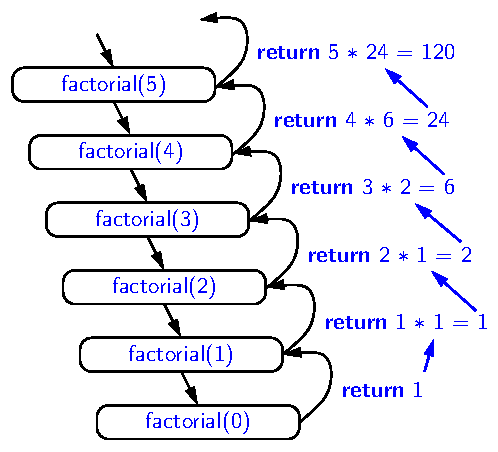
\includegraphics[width=7cm]{asp-02-pic01.pdf}
  \end{center}
}
\section[Engleski lenjir]{Engleski lenjir}
\frame{
  \frametitle{Primer rekurzije: ,,engleski lenjir``}
  \begin{itemize}
    \item odštampati crtice i brojeve tako da se dobije izgled lenjira
  \end{itemize}
  \begin{center}
    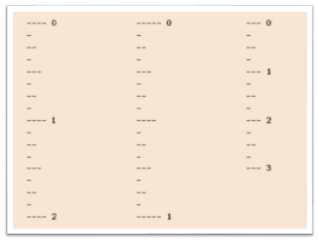
\includegraphics[width=8cm]{asp-02-pic02.png}
  \end{center}
}
\frame{
  \frametitle{Crtanje ,,engleskog lenjira``}
  \begin{itemize}
    \item \texttt{\myred{drawTicks}(length)}
    \item ulaz: dužina crtice
    \item izlaz: lenjir sa crticom date dužine u sredini i manji lenjiri sa leve
    i desne strane
  \end{itemize}
  \begin{center}
    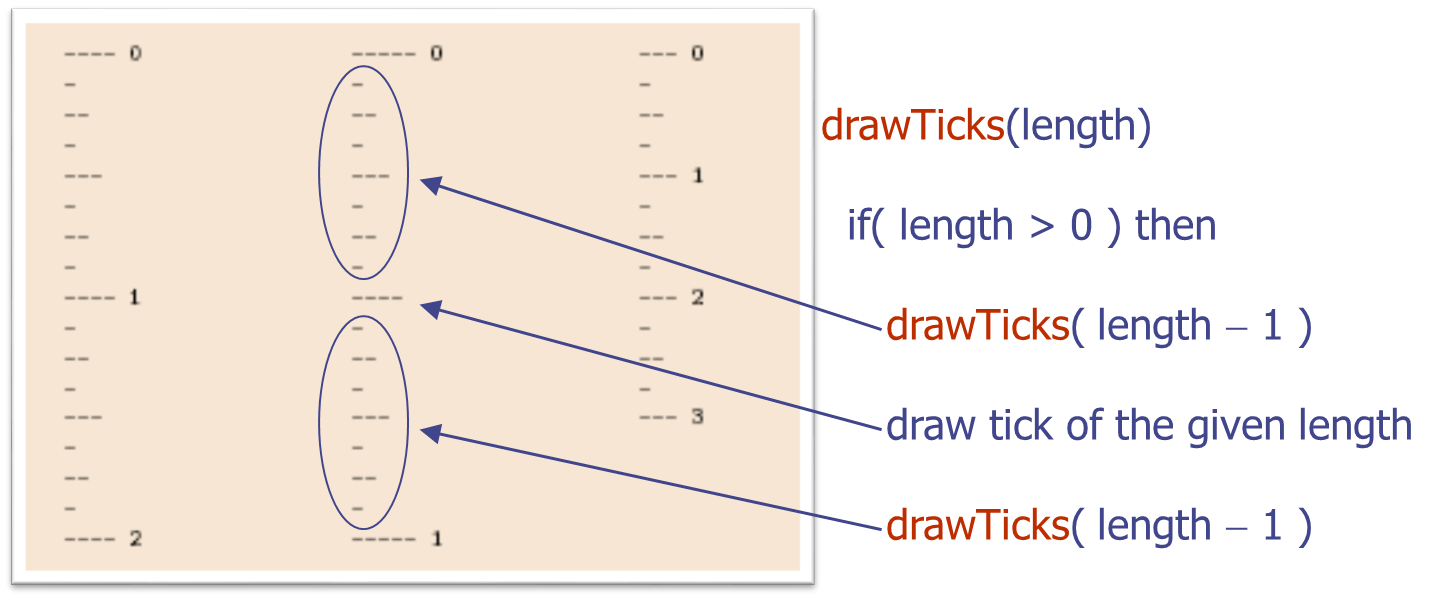
\includegraphics[width=11cm]{asp-02-pic03.png}
  \end{center}
}
\frame{
  \frametitle{Crtanje ,,engleskog lenjira``}
  \begin{itemize}
    \item interval sa centralnom crticom dužine $L \ge 1$ sastoji se od
    \begin{itemize}
      \item intervala sa centralnom crticom dužine $L-1$
      \item crtice dužine $L$
      \item intervala sa centralnom crticom dužine $L-1$
    \end{itemize}
  \end{itemize}
}
\frame{
  \frametitle{Crtanje ,,engleskog lenjira``}
  \begin{center}
    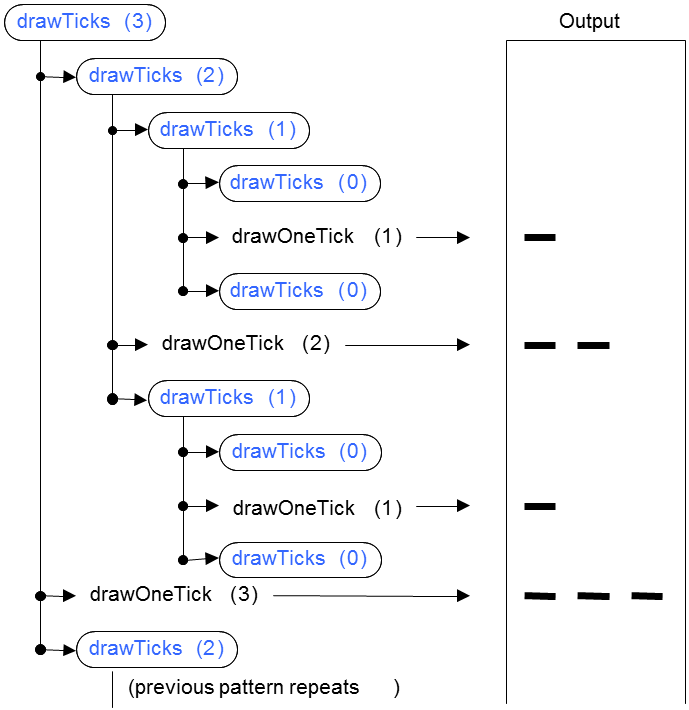
\includegraphics[width=7cm]{asp-02-pic04.png}
  \end{center}
}
\begin{frame}[fragile,shrink=10]
  \frametitle{Crtanje ,,engleskog lenjira``: Python implementacija}
\begin{minted}[linenos=false]{python}
def draw_line(tick_length, tick_label=''):
    """Draw one line with given tick length (followed by optional label)."""
    line = '-' * tick_length
    if tick_label:
        line += tick_label
    print(line)

def draw_interval(center_length):
    """Draw tick interval based upon a central tick length."""
    if center_length > 0:                 # recursively draw top ticks
        draw_interval(center_length - 1)  # draw center tick
        draw_line(center_length)          # recursively draw bottom ticks
        draw_interval(center_length - 1)

def draw_ruler(num_inches, major_length):
    """Draw English ruler with given number of inches, major tick length."""
    draw_line(major_length, '0')          # draw inch 0 line
    for j in range(1, 1+num_inches):
        draw_interval(major_length - 1)   # draw interior ticks for inch
        draw_line(major_length, str(j))   # draw inch j line and label
\end{minted}  
\end{frame}
\section[Binarna pretraga]{Binarna pretraga}
\begin{frame}[fragile,shrink=15]
  \frametitle{Binarna pretraga}
\begin{minted}[linenos=false]{python}
def binary_search(data, target, low, high):
  """Return True if target is found in indicated portion of a Python 
  list. The search only considers the portion from data[low] to 
  data[high] inclusive.
  """
  if low > high:
    return False                    # interval is empty; no match
  else:
    mid = (low + high) // 2
    if target == data[mid]:         # found a match
      return True
    elif target < data[mid]:
      # recur on the portion left of the middle
      return binary_search(data, target, low, mid - 1)
    else:
      # recur on the portion right of the middle
      return binary_search(data, target, mid + 1, high)
\end{minted}  
\end{frame}
\frame{
  \frametitle{Vizuelizacija binarne pretrage}
  \begin{itemize}
    \item \texttt{target == data[mid]} -- našli smo ga
    \item \texttt{target < data[mid]} -- ponavljamo pretragu u levoj
    polovini
    \item \texttt{target > data[mid]} -- ponavljamo pretragu u desnoj
    polovini
  \end{itemize}
  \begin{center}
    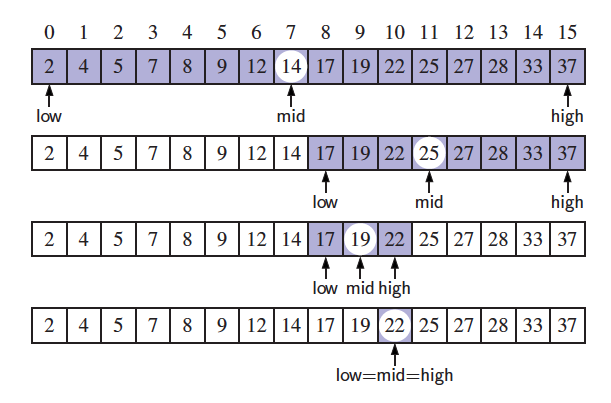
\includegraphics[width=8cm]{asp-02-pic05.png}
  \end{center}
}
\frame{
  \frametitle{Analiza binarne pretrage}
  \begin{itemize}
    \item radi u $O(\log n)$ vremenu
    \item veličina preostale liste je \texttt{high-low+1}
    \item posle jednog poređenja, to postaje
    $$ (mid-1)-low+1 = \left\lfloor{\frac{low+high}{2}}\right\rfloor \leq
    \frac{high-low+1}{2} $$ $$ high - (mid+1) + 1 = high -
    \left\lfloor{\frac{low+high}{2}}\right\rfloor \leq \frac{high-low+1}{2} $$
    \item $\Rightarrow$ svaki rekurzivni poziv deli region pretrage na pola;
    prema tome, može biti najviše $\log n$ nivoa
  \end{itemize}
}

\section[Linearna rekurzija]{Linearna rekurzija}
\frame{
  \frametitle{Linearna rekurzija}
  \begin{itemize}
    \item testiranje baznih slučajeva
    \begin{itemize}
      \item početi sa testiranjem baznih slučajeva (mora biti bar jedan)
      \item obrada baznog slučaja ne sme koristiti rekurziju
      \item svaki mogući lanac rekurzivnih poziva \myred{mora} se završiti
      dolaskom do baznog slučaja
    \end{itemize}
    \item rekurzivno jednom
    \begin{itemize}
      \item napraviti jedan rekurzivni poziv
      \item možemo napraviti grananje sa odlukom da se izabere jedan od mogućih
      rekurzivnih poziva
      \item svaki mogući rekurzivni poziv treba da se približi baznom slučaju
    \end{itemize}
  \end{itemize}
}

\begin{frame}[fragile]
  \frametitle{Primer linearne rekurzije}
\myred{LinearSum}($A$, $n$)
\begin{algorithmic}
\REQUIRE $A$: niz celih brojeva
\REQUIRE $n$: broj brojeva u nizu koje treba sabrati
\ENSURE suma prvih $n$ brojeva u $A$
\IF{$n = 1$}
  \RETURN $A[0]$
\ELSE
  \RETURN LinearSum($A$, $n-1$) + $A[n-1]$
\ENDIF
\end{algorithmic}
\end{frame}

\frame{
  \frametitle{Primer linearne rekurzije}
  \begin{center}
    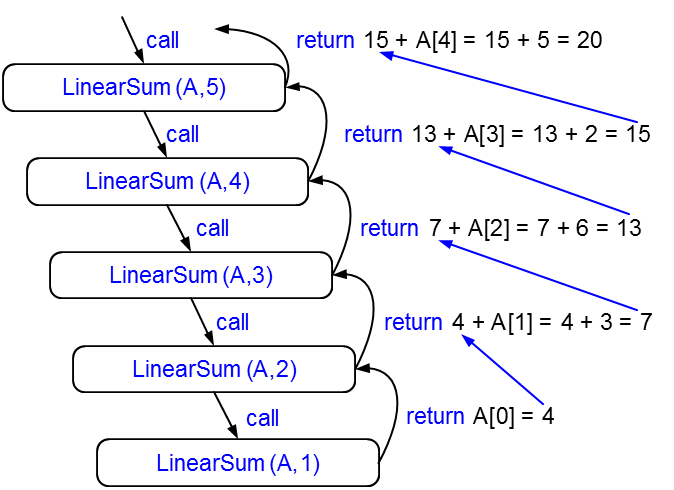
\includegraphics[width=8cm]{asp-02-pic06.png}
  \end{center}
}

\begin{frame}[fragile]
  \frametitle{Obrtanje redosleda u nizu}
\myred{ReverseArray}($A$, $i$, $j$)
\begin{algorithmic}
\REQUIRE $A$: niz brojeva
\REQUIRE $i$, $j$: nenegativni indeksi, $i<j$
\ENSURE obrnut redosled u $A$ počevši od indeksa $i$ do indeksa $j$
\IF{$i < j$}
  \STATE swap $A[i]$, $A[j]$
  \STATE ReverseArray($A$, $i+1$, $j-1$)
\ENDIF
\end{algorithmic}
\end{frame}
\begin{frame}[fragile]
  \frametitle{Definisanje elemenata za rekurziju}
  \begin{itemize}
    \item prilikom dizajniranja rekurzivnih funkcija važno je definisati ih tako da je rekurzija jednostavna
    \item ponekad to znači da treba definisati dodatne parametre funkcije
    \item na primer, definisali smo ReverseArray($A, i, j$) umesto ReverseArray($A$)
  \end{itemize}
\end{frame}
\begin{frame}[fragile]
  \frametitle{Definisanje elemenata za rekurziju}
  \begin{itemize}
    \item Python implementacija
  \end{itemize}
\begin{minted}[linenos=false]{python}
def reverse(S, start, stop):
  """Obrni elemente u isečku S[start:stop]."""
  # ako ima bar dva elementa
  if start < stop - 1:
    # zameni im mesta
    S[start], S[stop-1] = S[stop-1], S[start]
    # rekurzivno obrni ostatak
    reverse(S, start+1, stop-1)               
\end{minted}
\end{frame}

\begin{frame}[fragile]
  \frametitle{Stepenovanje}
  \begin{itemize}
    \item funkciju za stepenovanje $p(x,n) = x^n$ možemo definisati rekurzivno:
  \end{itemize}
  $$ p(x,n) = \left\{ \begin{array}{c l} 1 & \quad \text{ako } n=0 \\x\cdot p(x, n-1) & \quad \text{inače}\end{array}\right. $$
  \begin{itemize}
    \item na ovaj način ćemo dobiti funkciju koja radi u $O(n)$ vremenu (jer pravimo $n$ poziva)
    \item može li brže?
  \end{itemize}
\end{frame}

\begin{frame}[fragile]
  \frametitle{Stepenovanje}
  \begin{itemize}
    \item možemo napraviti brži linearno rekurzivan algoritam pomoću ponavljanog kvadriranja:
  \end{itemize}
  $$ p(x,n) = \left\{ \begin{array}{c l} 1 & \quad \text{ako je } x=0 \\x\cdot p(x, \frac{n-1}{2})^2 & \quad \text{ako je } x>0 \text{ neparan}\\p(x,n/2)^2 & \quad \text{ako je } x>0 \text{ paran} \end{array}\right. $$
  \begin{itemize}
    \item na primer: \\
    $ 2^4 = 2^{(4/2)2} = (2^{4/2})^2 = (2^2)^2 = 4^2 = 16 $ \\
    $ 2^5 = 2^{1+(4/2)2} = 2(2^{4/2})^2 = 2(2^2)^2 = 2(4^2) = 32 $ \\
    $ 2^6 = 2^{(6/2)2} = (2^{6/2})^2 = (2^3)^2 = 8^2 = 64 $ \\
    $ 2^7 = 2^{1+(6/2)2} = 2(2^{6/2})^2 = 2(2^3)^2 = 2(8^2) = 128$
  \end{itemize}
\end{frame}

\begin{frame}[fragile]
  \frametitle{Rekurzivno stepenovanje}
\myred{Power}($x, n$):
\begin{algorithmic}
\REQUIRE broj $x$ i njegov stepen $n$
\ENSURE vrednost $x^n$
\IF{$n=0$}
  \RETURN 1
\ENDIF
\IF{$n$ je paran}
  \STATE $y \leftarrow$ Power($x, (n-1)/2$) \COMMENT{\myred{svakim pozivom polovimo $n$}}
  \RETURN $x\cdot y\cdot y$
\ELSE
  \STATE $y \leftarrow$ Power($x, n/2$)
  \RETURN $y\cdot y$  \COMMENT{\myred{promenljiva umesto duplog poziva funkcije}}
\ENDIF  
\end{algorithmic}
\end{frame}

\begin{frame}[fragile]
  \frametitle{,,Repna`` rekurzija}
  \begin{itemize}
    \item kada je rekurzivni poziv poslednji korak u funkciji
    \item primer: ReverseArray($A, i, j$)
    \item lako se preradi u iterativni postupak
  \end{itemize}
\myred{IterativeReverseArray}($A, i, j$)
\begin{algorithmic}
\REQUIRE niz A i nenegativni indeksi $i$ i $j$, $i<j$
\ENSURE obrnut redosled elemenata u A počevši od indeksa $i$ do $j$
\WHILE{$i<j$}
  \STATE swap $A[i], A[j]$
  \STATE $i \leftarrow i + 1$
  \STATE $j \leftarrow j - 1$
\ENDWHILE
\end{algorithmic}
\end{frame}

\section[Binarna rekurzija]{Binarna rekurzija}
\begin{frame}[fragile]
  \frametitle{Binarna rekurzija}
  \begin{itemize}
    \item kada postoje \myred{dva} rekurzivna poziva za svaki bazni slučaj
    \item primer: engleski lenjir
  \end{itemize}
  \begin{center}
    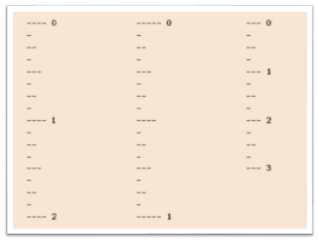
\includegraphics[width=5cm]{asp-02-pic02.png}
  \end{center}
\end{frame}

\begin{frame}[fragile]
  \frametitle{Binarna rekurzija: sumiranje elemenata}
\myred{BinarySum}($A, i, n$)
\begin{algorithmic}
\REQUIRE niz $A$ i celi brojevi $i$ i $n$
\ENSURE zbir $n$ brojeva iz $A$ počevši od $i$-tog
\IF{n=1}
  \RETURN $A[i]$
\ELSE
  \RETURN BinarySum($A, i, n/2$) + BinarySum($A, i+n/2, n/2$)
\ENDIF
\end{algorithmic}
  \begin{center}
    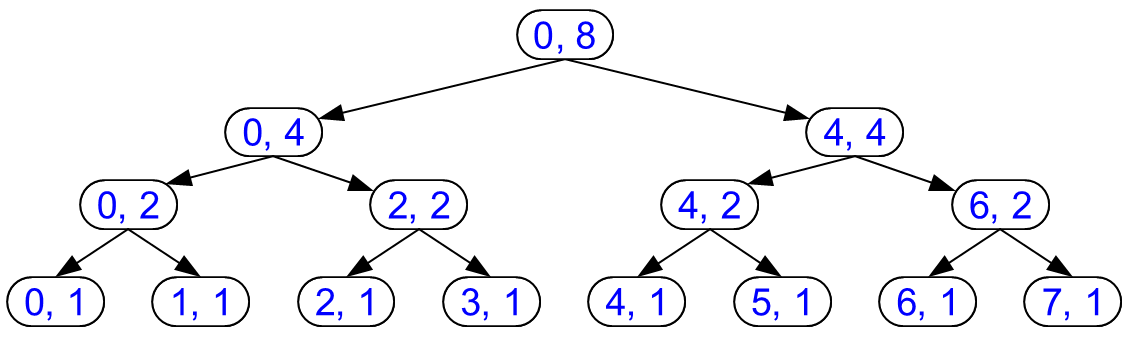
\includegraphics[width=10cm]{asp-02-pic07.png}
  \end{center}
\end{frame}

\begin{frame}[fragile]
  \frametitle{Fibonačijevi brojevi}
\begin{itemize}
  \item definišu se rekurzivno: \\
  $ F_0 = 0$ \\
  $ F_1 = 1$ \\
  $ F_i = F_{i-1} + F_{i-2} \quad $ za $i>1$ 
  \item rekurzivni algoritam (prvi pokušaj):
\end{itemize}
\myred{BinaryFib}($k$)
\begin{algorithmic}
\REQUIRE nenegativan ceo broj $k$
\ENSURE $k$-ti Fibonačijev broj $F_k$
\IF{$k\leq 1$}
  \RETURN $k$
\ELSE
  \RETURN BinaryFib($k-1$) + BinaryFib($k-2$)
\ENDIF
\end{algorithmic}
\end{frame}

\begin{frame}[fragile]
  \frametitle{Fibonačijevi brojevi}
\begin{itemize}
  \item neka je $n_k$ broj rekurzivnih poziva funkcije \myred{BinaryFib}($k$):
  \begin{itemize}
    \item $n_0 = 1$
    \item $n_1 = 1$
    \item $n_2 = n_1 + n_0 + 1 = 3$
    \item $n_3 = n_2 + n_1 + 1 = 5$
    \item $n_4 = n_3 + n_2 + 1 = 9$
    \item $n_5 = n_4 + n_3 + 1 = 15$
    \item $n_6 = n_5 + n_4 + 1 = 25$
    \item $n_7 = n_6 + n_5 + 1 = 41$
    \item $n_8 = n_7 + n_6 + 1 = 67$
  \end{itemize}
  \item $n_k$ se svaki drugi put više nego duplira!
  \item dakle, $n_k \geq 2^{k/2}$
  \item broj poziva raste \myred{eksponencijalno}!
\end{itemize}
\end{frame}

\begin{frame}[fragile]
  \frametitle{Fibonačijevi brojevi v2}
\begin{itemize}
  \item pomoću linearne rekurzije
\end{itemize}
\myred{LinearFib}($k$)
\begin{algorithmic}
\REQUIRE pozitivan ceo broj $k$
\ENSURE par Fibonačijevih brojeva $(F_k, F_{k-1})$
\IF{$k = 1$}
  \RETURN $(k, 0)$
\ELSE
  \STATE $(i, j) \leftarrow$ LinearFib($k-1$)
  \RETURN $(i+j, i)$
\ENDIF
\end{algorithmic}
\begin{itemize}
  \item ima samo $k-1$ rekurzivnih poziva!
\end{itemize}
\end{frame}

\section[Višestruka rekurzija]{Višestruka rekurzija}
\begin{frame}[fragile]
  \frametitle{Višestruka rekurzija}
\begin{itemize}
  \item primer problema: zagonetke sabiranja
  \begin{itemize}
    \item $pot + pan = bib$
    \item $dog + cat = pig$
    \item $boy + girl = baby$
  \end{itemize}
  \item višestruka rekurzija
  \item potencijalno pravi puno rekurzivnih poziva
  \item ne samo jedan ili dva
\end{itemize}
\end{frame}

\begin{frame}[fragile,shrink=12]
  \frametitle{Višestruka rekurzija}
\myred{PuzzleSolve}($k, S, U$)
\begin{algorithmic}
\REQUIRE ceo broj $k$, sekvenca $S$, skup $U$ (skup svih elemenata)
\ENSURE lista svih proširenja $S$ dužine $k$ korišćenjem elemenata iz $U$ bez ponavljanja
\FORALL{$e \in U$}
  \STATE ukloni $e$ iz $U$ \COMMENT {$e$ se sada koristi}
  \STATE dodaj $e$ na kraj $S$
  \IF{k = 1}
    \STATE test da li $S$ predstavlja rešenje
    \IF{$S$ predstavlja rešenje}
      \RETURN 'Solution found:', $S$
    \ENDIF
  \ELSE
    \STATE PuzzleSolve($k-1, S, U$)
    \STATE dodaj $e$ u $U$ \COMMENT{$e$ se više ne koristi}
    \STATE ukloni $e$ sa kraja $S$
  \ENDIF
\ENDFOR
\end{algorithmic}
\end{frame}

\begin{frame}[fragile]
  \frametitle{Višestruka rekurzija}
  $cbb + ba = abc$ \\
  $799 + 98 = 897$
  \begin{center}
    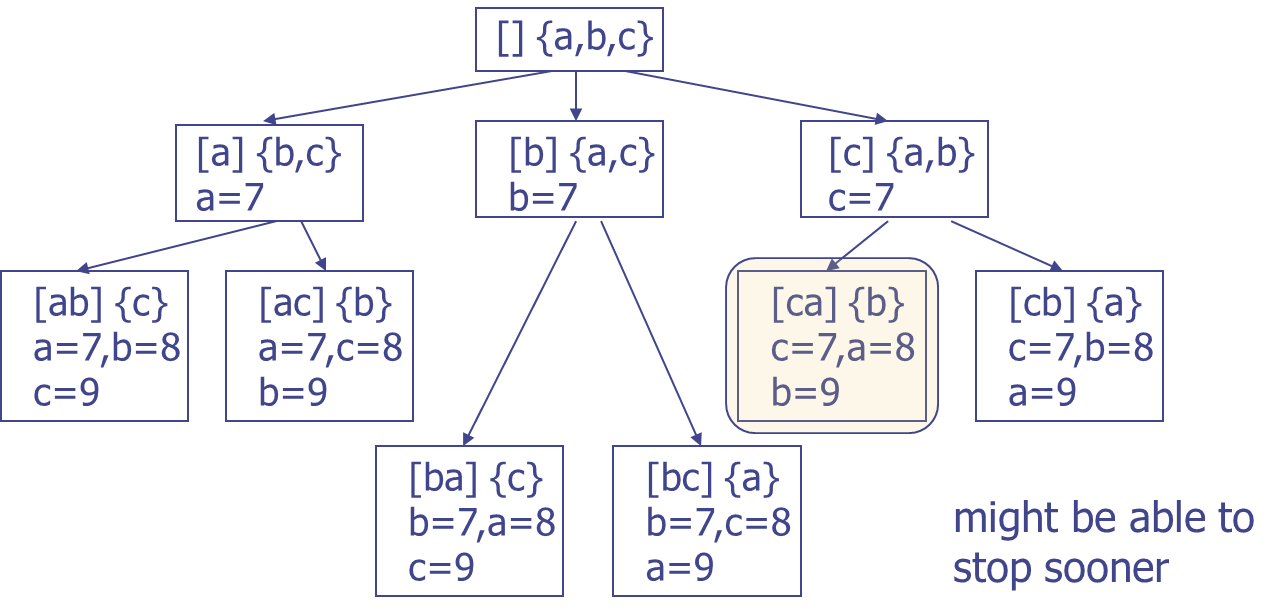
\includegraphics[width=10cm]{asp-02-pic08.png}
  \end{center}
\end{frame}

\begin{frame}[fragile]
  \frametitle{Višestruka rekurzija}
  \begin{center}
    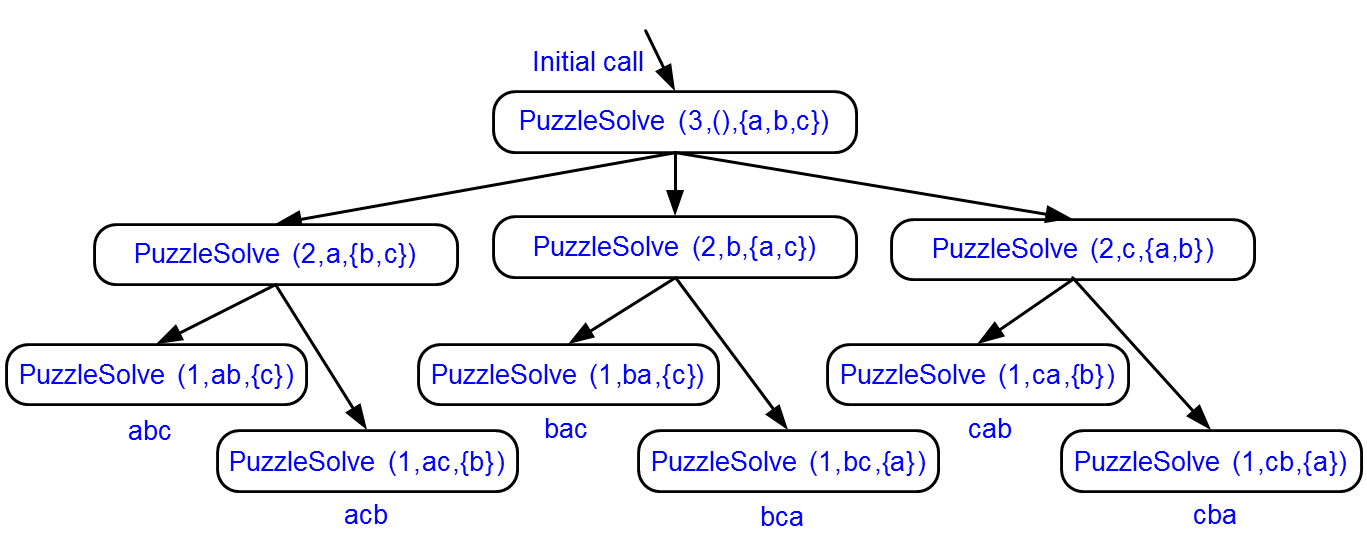
\includegraphics[width=11cm]{asp-02-pic09.png}
  \end{center}
\end{frame}

\end{document}
